\chapter{Religion, Authority, and Education I}

This chapter follows J. Krishnamurti's dialogue with Dr. Alan W. Anderson on religion, authority, and education. The source material belongs to J. Krishnamurti and the Krishnamurti Foundation Trust, with this course curated by LazyingArt LLC through Video2Book. There are no validated blackboard frames for this lecture, so the figures below are not reconstructions of visible board work. They are compact maps of the spoken argument, useful only where they preserve the sequence of distinctions: education and self-knowledge, religion and image, negation and reward, experience and recognition, knowledge and the living, authority and freedom.

\section{Education After Death, Love, And Fear}

Anderson opens by returning to the previous inquiry into death, living, and love. The next question is education: what really happens when teacher and student begin to look together? Why do fear, shock, and self-protection appear so quickly?

Krishnamurti widens the question at once. Education is not judged by whether it prepares one for employment, respectability, or social function. It is judged by whether it helps one understand living. If we are trained for jobs, money, pleasure, and entertainment, but remain unable to look into fear, death, thought, relationship, and inward emptiness, then something central has gone wrong.

The opening contrast can be kept as a working formula:
\begin{equation}
\text{education as training}
\;\not=\;
\text{education as understanding life}.
\end{equation}

This is not meant as a formal theorem. It is the lecture's initial pressure point. A person may be educated in the ordinary sense and still not know how to look at himself. That failure becomes most visible when one faces something real: fear, death, insecurity, or the collapse of a comforting belief.

From here Krishnamurti moves into religion. This is not a detour. Religion, as he examines it here, is one of the ways the unexamined mind escapes the emptiness of its own life. If daily living seems meaningless, thought creates symbols, rituals, and consolations. If death terrifies us, thought invents permanence. If we do not understand ourselves, we look for something or someone to do the work for us.

\section{Religion As The Image Made By Thought}

Krishnamurti begins with a very concrete image: a stone under a tree, a mark placed on it, flowers added, and soon the thing has become divine. The same movement, he says, continues in more elaborate forms: cathedrals, rituals, images, chants, and worship. The scale changes, but the structure remains the same.

The structure is:
\begin{equation}
\text{thought}
\longrightarrow
\text{image}
\longrightarrow
\text{worship of image}
\longrightarrow
\text{worship of what thought made}.
\end{equation}

The important point is that the mind then asks this image for security. It worships the Buddha, Christ, the guru, the father image, the saviour, or the ideal, but in Krishnamurti's analysis the image has been made by the human mind. So the worship looks outward while its object has been inwardly constructed.

\begin{figure}
\centering
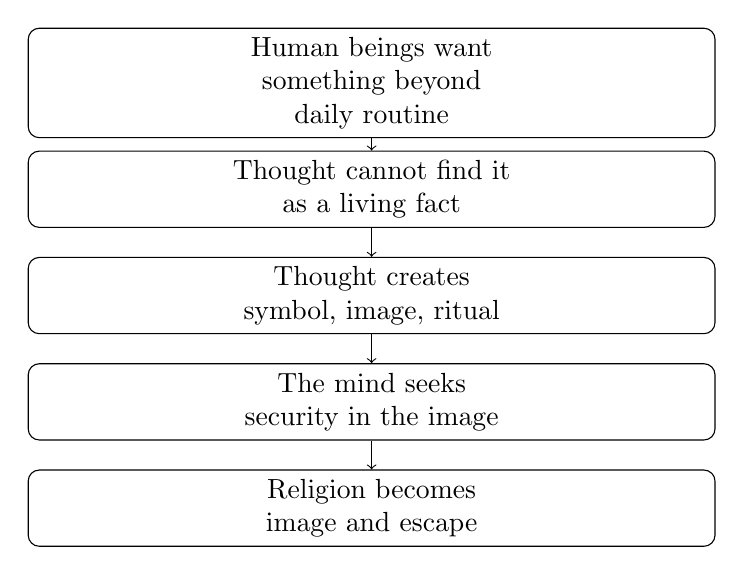
\begin{tikzpicture}
\node[draw, rounded corners, align=center, text width=0.70\linewidth] (a) at (0,0) {Human beings want\\something beyond\\daily routine};
\node[draw, rounded corners, align=center, text width=0.70\linewidth] (b) at (0,-1.35) {Thought cannot find it\\as a living fact};
\node[draw, rounded corners, align=center, text width=0.70\linewidth] (c) at (0,-2.70) {Thought creates\\symbol, image, ritual};
\node[draw, rounded corners, align=center, text width=0.70\linewidth] (d) at (0,-4.05) {The mind seeks\\security in the image};
\node[draw, rounded corners, align=center, text width=0.70\linewidth] (e) at (0,-5.40) {Religion becomes\\image and escape};
\draw[->] (a) -- (b);
\draw[->] (b) -- (c);
\draw[->] (c) -- (d);
\draw[->] (d) -- (e);
\end{tikzpicture}
\caption{A transcript-derived map of the image-making sequence. It is a conceptual reconstruction, not a redrawn blackboard figure.}
\end{figure}

This is why the lecture does not become a comparison of religions. Krishnamurti is not asking us to choose between traditions. He is asking whether the same principle is operating in all of them: thought makes an image, surrounds it with belief and ritual, and then depends on it for inward safety.

The next step is negation. If religion has become image, belief, superstition, personal worship, ritual, and tradition, what does it mean to put all that aside?

\subsection{Question \& Answer}

\paragraph{Question.}
Is negation a way of attaining something better?

\paragraph{Answer.}
No. Anderson notices the trap: one may say, ``I will negate all this in order to get something higher.'' Krishnamurti rejects that immediately. If negation is undertaken for reward, it is still desire. It is not negation.

The distinction is:
\begin{align}
\text{negation as pursuit}
&=
\text{denial for the sake of a better state},\\
\text{negation as perception}
&=
\text{seeing the false as false}.
\end{align}

The lecture's use of negation belongs to the second line. One does not first possess truth and then use it as a weapon against error. One sees the false clearly. In that seeing, the false has no further authority.

A compact relation is:
\begin{equation}
\text{clear perception of the false}
\longrightarrow
\text{the negation of the false}.
\end{equation}

The arrow matters. We should not turn this into a method. Krishnamurti is not giving a practice for becoming religious in a new way. He is saying that perception itself is action when the false is seen without reward, fear, or motive.

\section{The Tree, The Observer, And The Loss Of Direct Looking}

At this point Anderson brings in a classroom example. He had asked students to look at a tree. One young woman described her looking in a way that seemed direct and unblocked. Then he asked whether, while looking, she had been thinking of herself as looking. She hesitated. In that hesitation she began to fall out of the act.

Krishnamurti's response is brief and decisive: that is the observer.

This example is the pedagogical center of the lecture. It shows that the false is not only religious belief or ritual. It can be the subtle image of oneself in the act of seeing. A person looks; then the thought appears, ``I am looking,'' or ``I must say the right thing.'' The act is no longer simply looking. It is now watched, measured, defended, and reported by the self-image.

The sequence is:
\begin{equation}
\text{direct looking}
\longrightarrow
\text{self-reference}
\longrightarrow
\text{hesitation}
\longrightarrow
\text{loss of direct act}.
\end{equation}

\begin{proposition}
In Anderson's classroom example, the observer is not introduced as a separate inner entity. It is the movement of self-reference entering the act of perception.
\end{proposition}

\begin{proof}
The steps remain close to the example.
\begin{enumerate}
\item The student first describes looking at the tree without an obvious blockage between herself and the tree.
\item Anderson asks whether she had been thinking of herself as looking.
\item The question awakens self-reference.
\item The student begins to think of the classroom situation and of saying the right thing.
\item The direct relation to the tree is displaced by concern with the image of herself as the one who reports correctly.
\end{enumerate}
Thus the observer is not a theory added to the event. It is visible in the change from direct looking to self-conscious looking.
\end{proof}

Krishnamurti then returns to negation through this example. Negation can take place only when the mind sees the false. The student's hesitation is revealing because it shows the false not as an abstract doctrine, but as a small movement of self-protection in the act of learning.

\section{Experience, Recognition, And The Old}

Krishnamurti now says that one has to go more deeply into thought. Thought has built the technological world, but it has also built religious images, chants, cathedrals, masters, gurus, and father figures. Unless thought is understood, the same game will be played again in a different field.

Anderson then raises the word ``experience.'' People do not merely say they need awakening; they say they need the experience of awakening. They want an experience of God, an experience of the sacred, an experience that someone else claims to possess and can confer.

Krishnamurti's question is: why do we demand experience? We already have experiences of every kind: insult, flattery, incident, influence, pleasure, frustration. We are experiencing all the time. But we become bored with that and want a special experience.

\subsection{Question \& Answer}

\paragraph{Question.}
Can a spiritual experience be genuinely new if it is recognized as an experience?

\paragraph{Answer.}
Krishnamurti's answer is no. To know that I have had an experience, I must recognize it. Recognition implies that I already know what I am recognizing. Therefore the experience, insofar as it is recognized, belongs to the old.

\begin{proposition}
A recognized ``new'' experience is not new in Krishnamurti's sense.
\end{proposition}

\begin{proof}
We can write the argument as a short derivation.
\begin{enumerate}
\item I claim that I have had a special experience.
\item To make that claim, I must know that the experience occurred.
\item To know it occurred, I must recognize it.
\item Recognition depends on what is already known.
\item What depends on the already known is not the new.
\end{enumerate}
Therefore the recognized ``new'' experience is bound to memory, recognition, and the past.
\end{proof}

The compressed form is:
\begin{equation}
\text{experience known as experience}
\longrightarrow
\text{recognition}
\longrightarrow
\text{already known}
\longrightarrow
\text{not new}.
\end{equation}

This is the lecture's sharpest logical passage. It should remain stepwise. The point is not to deny ordinary experience. It is to expose the religious craving for a special experience, especially when that craving makes one dependent on someone who says, ``I know,'' ``I have experienced,'' or ``I can give this to you.''

\section{Beauty Or Gratification Through Beauty}

The inquiry into experience opens into beauty. Anderson mentions chant, cadence, Sanskrit invocation, euphoria, and somnolence. He also points out a subtle evasion: one may blame the music or the words as seductive, instead of seeing the self that wants to be seduced.

Krishnamurti's reply distinguishes beauty from gratification through beauty. Beauty, as he uses the word here, is connected with the abandonment of the self and the emptying of consciousness of its content. Gratification through beauty is different. It is the satisfaction, relief, sacred feeling, or inward comfort one may get from words, robes, incense, architecture, colored light, and religious atmosphere.

The distinction is:
\begin{align}
\text{beauty}
&\sim
\text{absence or emptying of the self},\\
\text{gratification through beauty}
&\sim
\text{satisfaction, relief, and sacred feeling}.
\end{align}

This distinction protects the passage from becoming an argument against music, architecture, or liturgy as objects. The point is not that chant or cathedrals are inherently corrupt. The point is that the self can use beauty as another experience, another refuge, another place to feel quiet and protected without understanding daily life.

\begin{table}
\centering
\begin{tabular}{p{0.42\linewidth} p{0.42\linewidth}}
\hline
Beauty without self & Gratification through beauty \\
\hline
Abandonment of the self & Satisfaction of the self \\
Emptying of consciousness of its content & Relief through words, robes, incense, architecture \\
Not dependent on religious trappings & Easily mistaken for sacredness \\
Bears on how one lives & Can remain separate from daily life \\
\hline
\end{tabular}
\caption{The lecture's distinction between beauty and gratification through beauty.}
\end{table}

Krishnamurti then compresses the matter into a severe statement: experience is a trap. That statement leads directly to the next term, ``knowledge.'' The experience that is sought is often called knowledge, and the one who claims to have it becomes an authority.

\section{Knowledge, Authority, And The Intermediary}

Krishnamurti asks what is meant when someone says, ``I know,'' especially in inward or spiritual matters. What is known, he says, is already past. It is gone, finished, dead. A living thing is moving; it is never the same. Therefore the living cannot be possessed as knowledge.

A compact form is:
\begin{equation}
\text{knowledge}
\sim
\text{the past},
\qquad
\text{the living}
\not\sim
\text{known possession}.
\end{equation}

This is not a rejection of practical knowledge. The target is the spiritual claim of possession: I know, I have experienced, I have knowledge, and I will give it to you. Krishnamurti calls this impudent because it turns the living into the already known and then asks others to obey.

The lecture now distinguishes practical authority from inward authority. We obey traffic rules. We may listen carefully to a doctor. But that is not the same as inwardly accepting a priest, guru, or intermediary who claims to know what we do not.

\begin{table}
\centering
\begin{tabular}{p{0.42\linewidth} p{0.42\linewidth}}
\hline
Practical authority & Inward authority \\
\hline
Law, road rules, practical order & Priest, guru, intermediary \\
Can be listened to watchfully & Often accepted through fear or despair \\
Does not require inward slavery & Claims spiritual knowledge or protection \\
Belongs to functional life & Invades freedom, intelligence, and inquiry \\
\hline
\end{tabular}
\caption{A small table preserving the lecture's contrast between practical and inward authority.}
\end{table}

Krishnamurti's question is pointed: why would a person reject political tyranny and yet accept spiritual tyranny? Why does the mind divide life this way? The answer unfolds through fear, loneliness, despair, ignorance, and the wish for someone else to do the inward work.

The dependency chain is:
\begin{equation}
\text{fear, loneliness, ignorance}
\longrightarrow
\text{acceptance of authority}
\longrightarrow
\text{obedience}
\longrightarrow
\text{loss of inward freedom}.
\end{equation}

Anderson adds an important bridge from the earlier inquiry into fear. The infant has need: to feed, to be held, to be cared for. In that radical need there is no intermediary of the infant's own contrivance. Later, as one grows older, thought begins to imagine the source of the meeting of need. An image is interposed between danger and action.

We should keep this cautious, since the formulation is Anderson's and Krishnamurti agrees to it. The contrast is:
\begin{align}
\text{radical need}
&\longrightarrow
\text{immediate action},\\
\text{sense of danger}
&\longrightarrow
\text{image or intermediary}
\longrightarrow
\text{deferred or distorted action}.
\end{align}

\begin{figure}
\centering
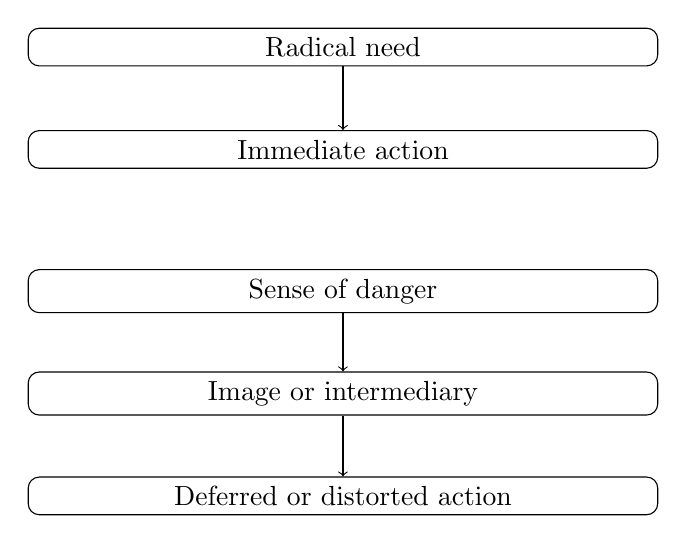
\begin{tikzpicture}
\node[draw, rounded corners, align=center, text width=0.64\linewidth] (a) at (0,0) {Radical need};
\node[draw, rounded corners, align=center, text width=0.64\linewidth] (b) at (0,-1.30) {Immediate action};

\node[draw, rounded corners, align=center, text width=0.64\linewidth] (c) at (0,-3.10) {Sense of danger};
\node[draw, rounded corners, align=center, text width=0.64\linewidth] (d) at (0,-4.40) {Image or intermediary};
\node[draw, rounded corners, align=center, text width=0.64\linewidth] (e) at (0,-5.70) {Deferred or distorted action};

\draw[->] (a) -- (b);
\draw[->] (c) -- (d);
\draw[->] (d) -- (e);
\end{tikzpicture}
\caption{A narrow reconstruction of Anderson's contrast between immediate need and the later insertion of image or intermediary.}
\end{figure}

The practical consequence is severe. Inwardly we may stop reasoning exactly where freedom, intelligence, and reasoning are most needed. Someone tells us what to do; we repeat. Tradition, repetition, discipline, and obedience then take the place of inquiry.

\section{Education Without Authority}

The final movement returns to education. If education as it is trains thought, memory, acceptance, obedience, and reaction, can there be an education in which there is no psychological authority?

\subsection{Question \& Answer}

\paragraph{Question.}
Can there be education without authority?

\paragraph{Answer.}
The dialogue does not answer by designing a system. Anderson says yes, but his yes comes from experiment: a classroom in which students are invited to look together, not to do what the teacher says. The teacher and student question together. They try to grasp without turning that grasping into the familiar effort to please, perform, or obey.

This is the educational form of the whole lecture. The teacher is not the one who possesses knowledge and transfers it to the ignorant. The teacher and student share inquiry. But that sharing exposes the next difficulty: students trained in effort, obedience, and correctness may be shocked when authority is suspended.

The movement can be kept as:
\begin{equation}
\text{authority-free inquiry}
\longrightarrow
\text{shock}
\longrightarrow
\text{attention}
\longrightarrow
\text{hesitation}.
\end{equation}

Anderson describes the students as standing at the edge of an abyss, like water reaching the lip of a cup and not quite spilling over. Krishnamurti, drawing on long experience with schools, says that when students are asked about freedom, authority, and acceptance, they are often lost. They may want slavery, or they may reject one form of slavery while accepting another.

So the lecture ends with an unfinished but precise question. Can learning occur without turning the teacher into an intermediary? Can attention operate without effort becoming another form of self-concern? Can the student meet the moment of hesitation without retreating into obedience?

\section{Summary}

The chapter has one continuous movement. Education is questioned because it has not taught us to understand life. Religion is questioned because thought creates images and then seeks security in them. Negation is clarified as seeing the false, not pursuing a reward. Anderson's tree example shows the observer entering the act of looking. The demand for experience is examined through recognition: what is recognized is already known, and therefore not new. Beauty is distinguished from gratification through beauty. Knowledge is questioned where it claims possession of the living. Authority is traced to fear, loneliness, ignorance, repetition, and the wish for someone else to do the inward work.

The final question remains open:
\begin{equation}
\text{Can teacher and student inquire together}
\quad
\text{without psychological authority?}
\end{equation}

That question carries the inquiry forward. It belongs in Part III because it moves toward attention, freedom, education, and transformation, while still carrying the earlier investigations of fear, death, desire, image, and relationship inside it.